\chapter{Einleitung}  \label{einleitung}

%motivation
 Die Herstellung von Produktabbildungen für Werbung und Kataloge erfolgt oft in einem Fotostudio unter Einsatz einer sehr aufwändigen Beleuchtungstechnik.
 Das Erscheinungsbild eines Gegenstandes wird nämlich nicht nur durch die Form und das Material bestimmt, sondern hängt auch davon ab wie es beleuchtet wird.
  Dies ist insbesondere bei spiegelnden oder transparenten Materialien der Fall: Ihr Aussehen wird weitgehend durch die einfallende Beleuchtung bestimmt, da sich an ihnen die gesamte Umgebung reflektiert oder bricht.
  Das Licht, das von einer realen Umgebung ausgeht, besitzt sehr feine Details und einen hohen Kontrast, weshalb es in einem Fotostudio nicht ohne Weiteres erzeugt werden kann.
  Objekte dieser Art werden darum in der Regel in einem weißen Fotozelt fotografiert, das eine gleichmäßige, diffuse Beleuchtung erzeugt. 
  
  Soll das Objekt jedoch unter eine realen Beleuchtung abgebildet werden, so muss man es entweder direkt unter einer realen Umgebungsbeleuchtung fotografiert, oder mit Hilfe eines Computermodells rendern.
  Das Rendern ist oft die einfachste und kostengünstigste Möglichkeit, es erfordert jedoch dass eine Beschreibung der Form und der Materialeigenschaften vorliegt, was nicht immer der Fall ist.
  Bei komplizierten, natürlichen  Objekten ist dies auch teilweise gar nicht möglich, da die tatsächliche Form aber auch das Verhalten des Lichts im Material nicht bekannt ist, und auch nicht ohne großen Aufwand gemessen werden kann. 
  Aus diesem Grund wird ein Verfahren benötigt, mit dem man solche Materialien in einem Fotostudio kostengünstig und mit hoher Auflösung beleuchten kann.

%these  
  %Das Erzeugen einer hochauflösende Beleuchtung erfordert sehr viele individuell steuerbare Lichtquellen die rund um das Objekt angeordnet sind.
  Eine hochauflösende Beleuchtung erfordert sehr viele, individuell steuerbare Lichtquellen, die rund um das Objekt angeordnet sind. 
  Hierzu sind Flachbildschirme ideal geeignet, denn sie bestehen aus einem Array von hundert tausenden einzelnen, farbigen Lichtpunkten und lassen sich präzise und mit hoher Frequenz ansteuern.
  Mit einem einzelnen Bildschirm lässt sich aber nur ein Teil einer umschließenden Beleuchtung erzeugen. 
  Bewegt man ihn an viele Positionen rund um das Objekt, so kann man eine vollständige Beleuchtung stückweise erzeugen.
  Fotografiert man die Szene unter vielen Teilbeleuchtungen, so kann man die Aufnahmen im Anschluss kombinieren und erhält eine vollständig beleuchtete Szene.
 

%  Damit dies möglich ist muss die Position der Bildschirmpixel im Raum zu jedem Zeitpunkt bekannt sein.
  Für eine realistische Beleuchtung wird Licht mit einem hohen Kontrastverhältnis benötigt.
  Gewöhnliche Bildschirme, wie sie in den meisten portablen Geräten verbaut sind, besitzen jedoch nur einen geringen Dynamikbereich, der weitaus kleiner als der einer realen Beleuchtung ist.
  Sie können also nicht ohne Weiteres direkt für eine fotografische Beleuchtung verwendet werden.
  Mit Wissen über die Funktionsweise eines Bildschirms ist es jedoch möglich, seinen Dynamikbereich durch eine zeitvariante Bildsequenz zu erhöhen.



   
\section{Aufgabenstellung}  \label{aufgabenstellung}
  In dieser Arbeit soll untersucht werden, wie sich ein Bildschirm mit handelsüblichen Kontrast zum Erzeugen einer fotografischen Beleuchtung einsetzen lässt.
  Die Beleuchtung soll dabei neben einer hohen Auflösung auch einen großen Dynamikbereich besitzen.
  Das Ziel ist es, dass der Bildschirm von Hand rund um die Szene bewegt werden kann. Seine Koordinaten sollen dabei automatisch durch eine daran befestigte Kamera bestimmt werden.
  An jeder Position soll, wie in Abbildung \ref{fig:beleuchtung} dargestellt, ein Ausschnitt ($B_1$) einer vorgegebenen Beleuchtung erzeugt und fotografiert werden. 
 Die einzelnen Teilbeleuchtungen müssen dabei so erzeugt werden, dass sich die einzelnen Aufnahmen im Anschluss zu einer korrekten, vollständigen Beleuchtung zusammenführen lassen.
  Es soll also eine zusammenhängende Lichtfläche enstehen, weshalb die Überlappung zu aufeinander folgende Teilbeleuchtungen ($B_2$, $B_3$) beachtet werden muss: Der Bildschirm darf immer nur das Licht emittieren, das noch nicht von einer vorangegangenen Teilbeleuchtung hergestellt wurde.

  \begin{figure}[H]
    \centering
    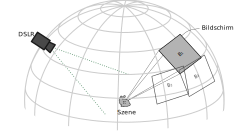
\includegraphics[width=0.8\linewidth]{../graphics/einleitung/beleuchtung.svg}
    \caption[Eine reale Szene mit einen Bildschirm beleuchten]{Ein Objekt wird mit einem Bildschirm beleuchtet, der an mehrere Stellen $B_1-B_3$ bewegt wird und dort jeweils einen Teil der einfallenden Beleuchtung erzeugt. }
    \label{fig:beleuchtung}
   \end{figure}


  Der Bildschirm und die Kameras müssen dazu sowohl radiometrisch als auch geometrisch kalibriert werden, sodass mit den Bildschirmpixeln gezielt eine einfallende Strahldichteverteilung erzeugt werden kann.
  Die Beleuchtungsberechnung  soll automatisiert erfolgen,  sodass der Benutzer den Bildschirm lediglich an mehrere Positionen, wie auf einer Halbkugel, rund um das Objekt bewegen muss.
  Da der Dynamikbereich eines herkömmlichen Bildschirms klein ist, soll des weiteren untersucht werden, ob und wie man eine zeitvariante Sequenz dazu verwenden kann, ihn zu vergrößern, sodass eine natürliche Umgebungsbeleuchtung hergestellt werden kann.
  Dabei sollen keine teuren Messgeräte oder aufwändige  Aufbauten eingesetzt werden.

  
\section{Gliederung}  \label{gliederung}
  
Die Arbeit ist in folgender Weise gegliedert:
\begin{description}
   \item[2. Grundlagen] \hfill \\
       Erklärt die wichtigsten Grundlagen, die zum Verständnis der Arbeit benötigt werden:
       Die verwendeten mathematischen Notationen; Licht und distante Beleuchtung, Cube-Maps, Dynamikbereich von Licht; das Pinhole-Modell für Kameras sowie seine Anwendung bei der Positionsbestimmung;  aktuelle Bildschirmtechnologien  und ihre Eigenschaften mit Hinblick auf die Beleuchtungserzeugung.

  \item[3. Verwandte Arbeiten] \hfill \\
       Verwandte Arbeiten die sich mit der Beleuchtung von Szenen auseinandersetzen.

  \item[4. Modell und Kalibrierung] \hfill \\
       Hier wird das System und alle Komponenten zuerst vorgestellt, dann radiometrisch sowie geometrisch modelliert und anschließend kalibriert.
  
  \item[5. Tracking-Stage] \hfill \\
      Damit die Position des Bildschirms mit einer Kamera bestimmt werden kann, müssen geometrische Marker um die Szene angeordnet werden. Dieser Aufbau wird als ``Tracking-Stage'' bezeichnet.
      In diesem Kapitel wird erklärt wie die Markierungen ausgewählt und aufgebaut wurden.
      Zum Abschluss wird die Genauigkeit der Positionsberechnung evaluiert.
       
      
  \item[6. Beleuchtung] \hfill \\
       Der Kernpunkt der Arbeit: Es wird gezeigt, wie mit einem radiometrisch kalibrierten Bildschirm ein Teil einer vorgegebenen Beleuchtung erzeugt werden kann.
       Daraufhin wird die Theorie hinter der zeitvarianten Sequenz erklärt, und gezeigt, dass es damit möglich ist das Kontrastverhältnis zu erhöhen.
      Im Anschluss wird ein Verfahren vorgestellt, das es einen Benutzer ermöglicht eine zusammenhängende, nahezu vollständige Beleuchtung mit einem handgehaltenen Bildschirm zu erzeugen.
       Eine Evaluation der einzelnen Aspekte des Verfahrens bildet den Abschluss des Kapitels.
      
  \item[7. Ergebnisse] \hfill \\
       Erzeugen einer vollständigen und einer HDR-Beleuchtung mit dem vorgestellten Verfrahren, Diskussion der Ergebnisse.

  \item[8. Abschluss] \hfill \\
       Die Zusammenfassung der Arbeit und ein Ausblick auf mögliche Erweiterungen des Verfahrens.

\end{description}
